\begin{homeworkProblem}
\textbf{5x5 Grid World(Example 3.5 Gridworld in the book “Reinforcement Learning: An Introduction” , the second edition)}

(a) Find the state values under the uniform random policy with both theoretical method and iterative policy evaluation method.
\begin{figure}[h]
    \centering
    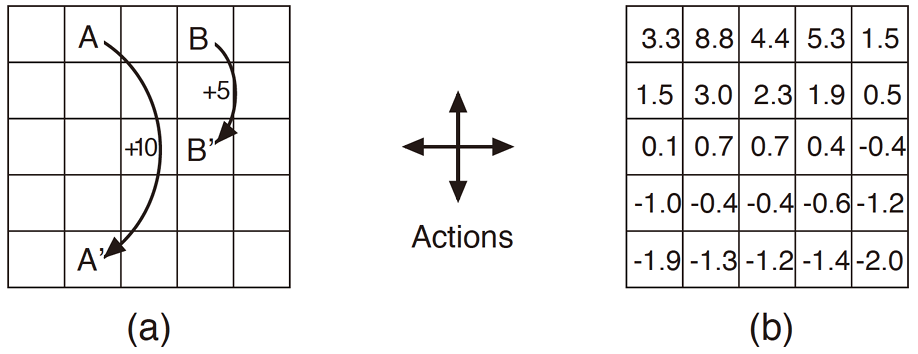
\includegraphics[width=0.5\textwidth]{./figure/grid1.png}
\end{figure}

(b) Reproduce the optimal state values, optimal state-action values, and optimal policy with theoretical method, policy iteration method and value iteration method.
\begin{figure}[h]
    \centering
    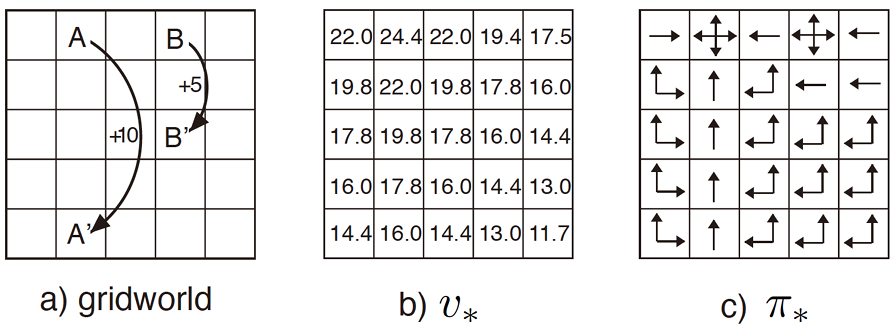
\includegraphics[width=0.5\textwidth]{./figure/grid2.png}
\end{figure}

\solution

In the book “Reinforcement Learning: An Introduction” , the second edition, Example 3.5 Gridworld. The setting is that in each cell, four actions are possible: north, south, east and west. Actions that would take the agent off the grid leave its location unchanged, but also result in a reward of -1. Other actions result in a reward of 0, except those that move the agent out of the special states A and B. From state A, all four actions yield a reward of +10 and take the agent to A'. From state B, all actions yield a reward of +5 and take the agent to B'.

The discount factor is set to be $\gamma=0.9$. Let the state value function under policy $\pi$ be $v_{\pi}(s)$. The action space is $\A=\text{\{north, south, east, west\}}$, and the state space is ordered by the position of the cells, from left to right, from up to down: $\mS=\{s_1,\cdots,s_{25}\}$, additionally, $s_2=A, s_4=B, s_{14}=B', s_{22}=A'$. The reward $\R$ is defined above, and the transition probability $\mP$ is deterministic, i.e. 1 if it suit the transition policy, 0 otherwise. So when know $s,a$, we can get the unique $s'$, thus we can get the reward:
$$\R_s^a=\begin{cases}
-1 & \text{if } s=s' \\
10 & \text{if } s=A, s'=A' \\
5 & \text{if } s=B, s'=B' \\
0 & \text{otherwise}
\end{cases}$$
The codes for (a), (b) could be found in the `hw5\_code.ipynb' file.

(a) From what we have learned, the Bellman Expectation Equation for $v_{\pi}$ is
$$v_{\pi}(s) = \sum_{a \in \A}\pi(a|s)\left(\R_s^a + \gamma \sum_{s' \in \mS} \mP_{s,s'}^a v_{\pi}(s)\right)$$
We can re-write is into the matrix form:
$$v_{\pi} = \R^{\pi} + \gamma \mP^{\pi}v_{\pi}$$
So from the definition
$$\R_s^{\pi}=\E\left[R_{t+1}|S_t=s\right]=\sum_{a \in \A}\sum_{s'\in\mS} \mP_{s,s'}^a\R_s^a=\dfrac{1}{4}\sum_{a\in\A} \R_s^a$$
So we can get
\begin{align*}
\R^{\pi} &= \left(\R_{s_1}^{\pi},\cdots,\R_{s_{25}}^{\pi}\right)^{\top} \\
\mP^{\pi} &= \left(\sum_{a\in\A}\mP_s^{a}\right)_{s,s': \text{ if $s$ could reach $s'$ through $a$}}
\end{align*}
And we can get $\R^{\pi}, \mP^{\pi}$ through coding, the numerical results are shown below.
\begin{figure}[h]
    \centering
    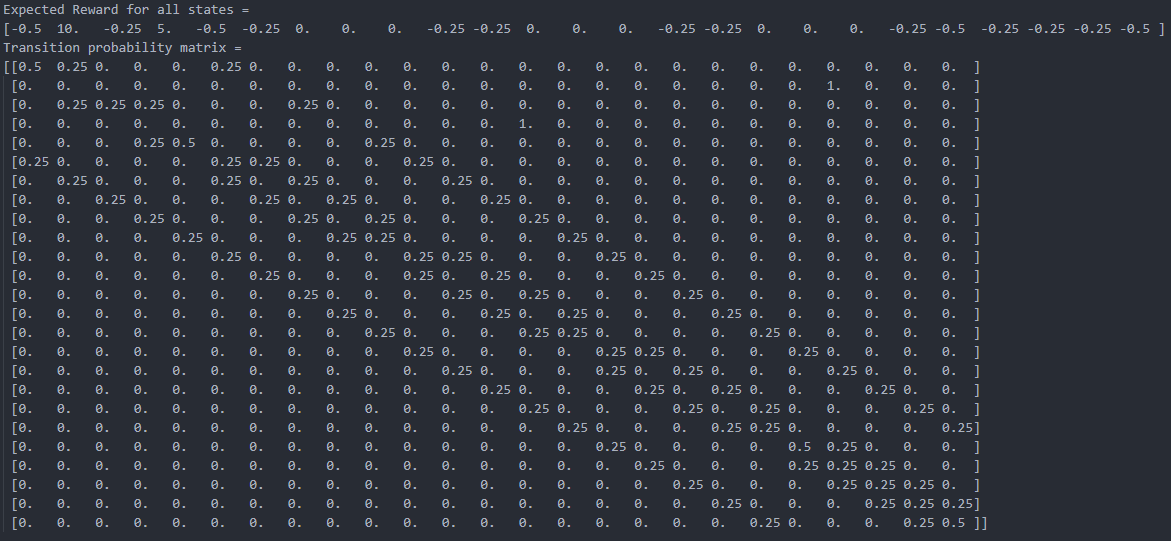
\includegraphics[width=\textwidth]{./figure/p3_output/uniform/theoritical_output.png}
\end{figure}

1. Theoretical method: \\
Using the matrices above, we can use the matrix form to get the theoretical state values by
$$v_{\pi} = \left(I-\gamma \mP^{\pi}\right)^{-1}\R^{\pi}$$
The result is shown as follows:
\begin{figure}[h]
    \centering
    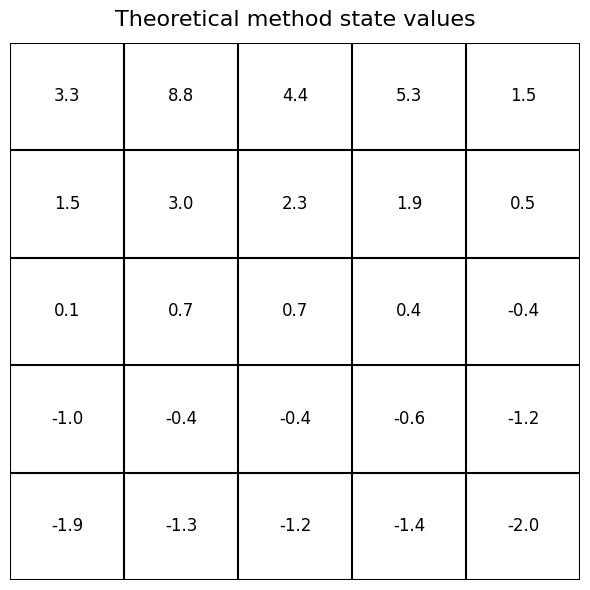
\includegraphics[width=0.4\textwidth]{./figure/p3_output/uniform/theoritical_values.png}
\end{figure}

2. Iterative policy evaluation method: \\
Directly apply the Bellman Expectation Equation iteratively, and use the assignment operator to update the state values. Here we regard the update using synchronous backups, i.e.
$$v_{\pi}^{k+1} = \R^{\pi} + \gamma \mP^{\pi}v_{\pi}^k$$
Define $\Delta$ as the maximum difference between the two iterations, i.e.
$$\Delta = \max_{s \in \mS}|v_{\pi}^{k+1}(s) - v_{\pi}^k(s)|$$
Initially, we set $v_{\pi}^0 = \mathbf{0}$. And we set a threshold $\epsilon=10^{-3}$, and stop the iteration when $\Delta < \epsilon$. The result is shown below. Which totally used $26$ iterations to converge.
\begin{figure}[h]
    \centering
    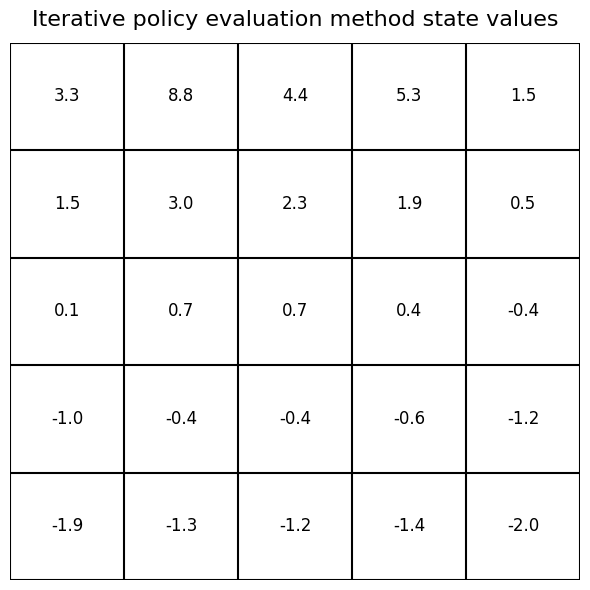
\includegraphics[width=0.35\textwidth]{./figure/p3_output/uniform/iterative_values.png}
\end{figure}

(b) Let $v_*(s)$ be the optimal state value function, and $q_*(s,a)$ be the optimal state-action value function. The Bellman Optimality Equation is:
\begin{align*}
v_*(s) &= \max_{a \in \A}\left(\R_s^a + \gamma \sum_{s' \in \mS} \mP_{s,s'}^a v_*(s')\right) \\
q_*(s,a) &= \R_s^a + \gamma \sum_{s' \in \mS} \mP_{s,s'}^a v_*(s')
\end{align*}
Where $\mP_{s,s'}^a$ is deterministic, as a valid transition has probability 1, and 0 otherwise. And $\R_s^a$ is defined above. So we can use the Bellman Optimality Equations to get the optimal state values $v_*(s)$ and the optimal state-action values $q_*(s,a)$. Since there might has more than one optimal action, we can define the optimal action set $\A(s)=\argmax\limits_{a \in \A} q_*(s,a)$. So the optimal policy $\pi^*$ is defined as:
$$\pi_*(a|s)=\begin{cases}
\dfrac{1}{|\A(s)|} & \text{if } a\in \A(s) \\
0 & \text{otherwise}
\end{cases}$$
Thus, we could get the optimal state value function $v_*(s)$ with different methods, then get optimal state-action value function $q_*(s,a)$ using $v_*(s)$ and final get the optimal policy $\pi^*(a|s)$ using $q_*(s,a)$.

1. Theoretical method: \\
We can re-write the definition of $v_*(s)$ into the an inequality form:
\begin{align*}
v_*(s) = \max_{a \in \A}\left(\R_s^a + \gamma \sum_{s' \in \mS} \mP_{s,s'}^a v_*(s')\right)
&\Rightarrow v_*(s) \geq \R_s^a + \gamma \sum_{s' \in \mS} \mP_{s,s'}^a v_*(s')\ \ \forall a\in A \\
&\Rightarrow -v_*(s) + \gamma \sum_{s' \in \mS} \mP_{s,s'}^a v_*(s') \leq -\R_s^a\ \ \forall a\in A
\end{align*}
So the Bellman Optimality Equation could be re-written into a set of inequality constrains. As we known of the basic knowledge of convex optimization, the optimal solution must be lying on the inconstraint set for the Linear Programming problem, thus we can add a linear objective function to ensure the inequality constrains try to be equal. So the final LP problem is:
\begin{align*}
\min_{v} &\qquad\quad \sum_{s \in \mS} v(s) \\
\text{s.t.} &\ -v(s) + \gamma \sum_{s' \in \mS} \mP_{s,s'}^a v(s') \leq -\R_s^a\ \ \forall s\in\mS, a\in \A
\end{align*}
Thus, solve the LP problem with optimizers, we can get the theoritical optimal state values, optimal state-action values and optimal policy. The result is shown below:
\begin{figure}[h]
    \centering
    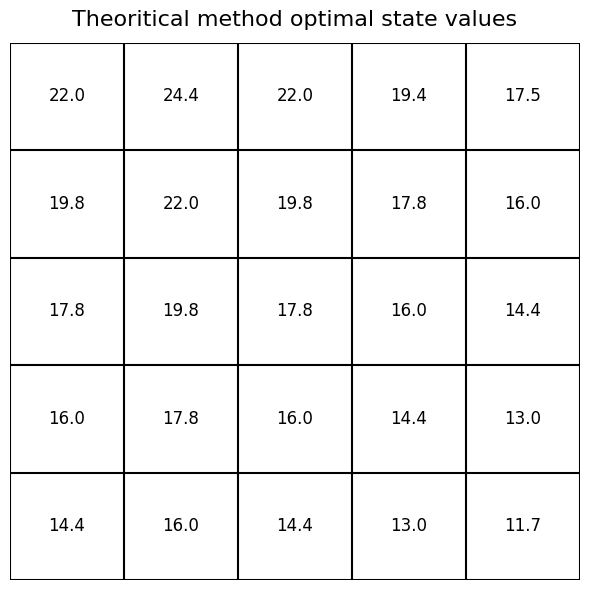
\includegraphics[width=0.48\textwidth]{./figure/p3_output/optimal/theoretical/V_value.png}
\end{figure}
\begin{figure}[h]
    \centering
    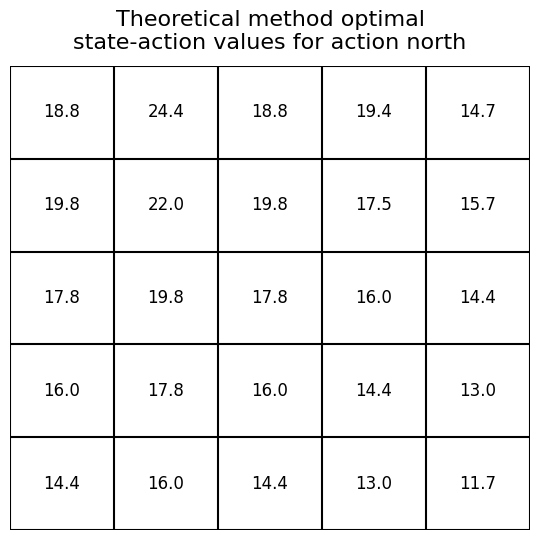
\includegraphics[width=0.48\textwidth]{./figure/p3_output/optimal/theoretical/Q_north.png}
    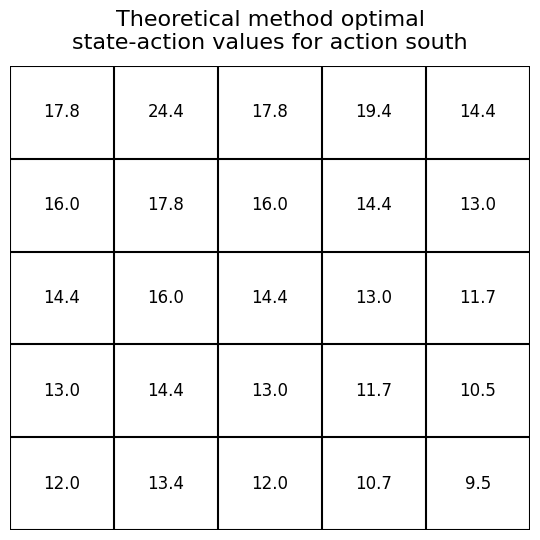
\includegraphics[width=0.48\textwidth]{./figure/p3_output/optimal/theoretical/Q_south.png}
\end{figure}
\begin{figure}[h]
    \centering
    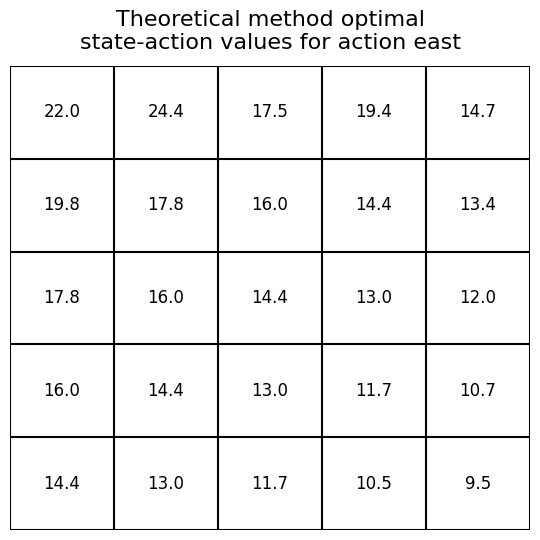
\includegraphics[width=0.48\textwidth]{./figure/p3_output/optimal/theoretical/Q_east.png}
    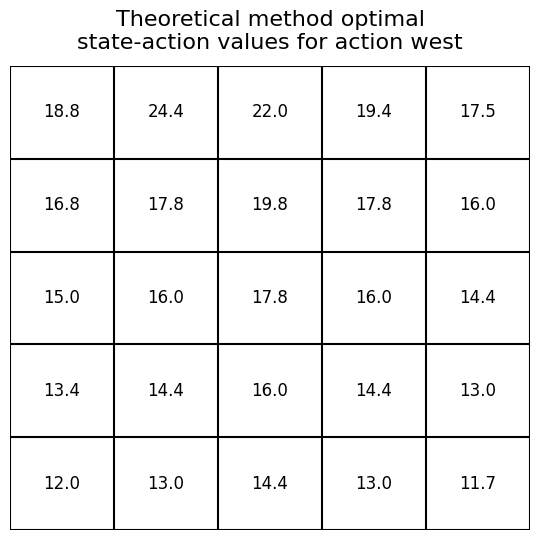
\includegraphics[width=0.48\textwidth]{./figure/p3_output/optimal/theoretical/Q_west.png}
\end{figure}
\begin{figure}[!htbp]
    \centering
    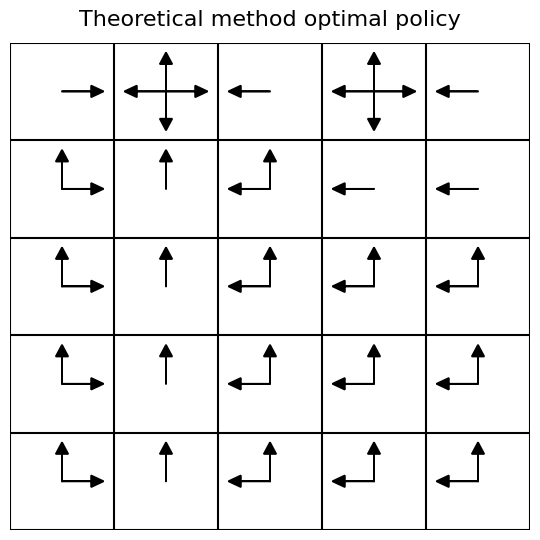
\includegraphics[width=0.4\textwidth]{./figure/p3_output/optimal/theoretical/policy.png}
    \vspace{-0.5cm}
\end{figure}

2. Policy iteration method: \\
We can applying policy iteration method through the following pseudocode to get $v_*(s)$ and $\pi_*(s)$, then get $q_*(s,a)$ by Bellman Optimality Equation using $v_*(s)$:
\begin{figure}[!htbp]
    \centering
    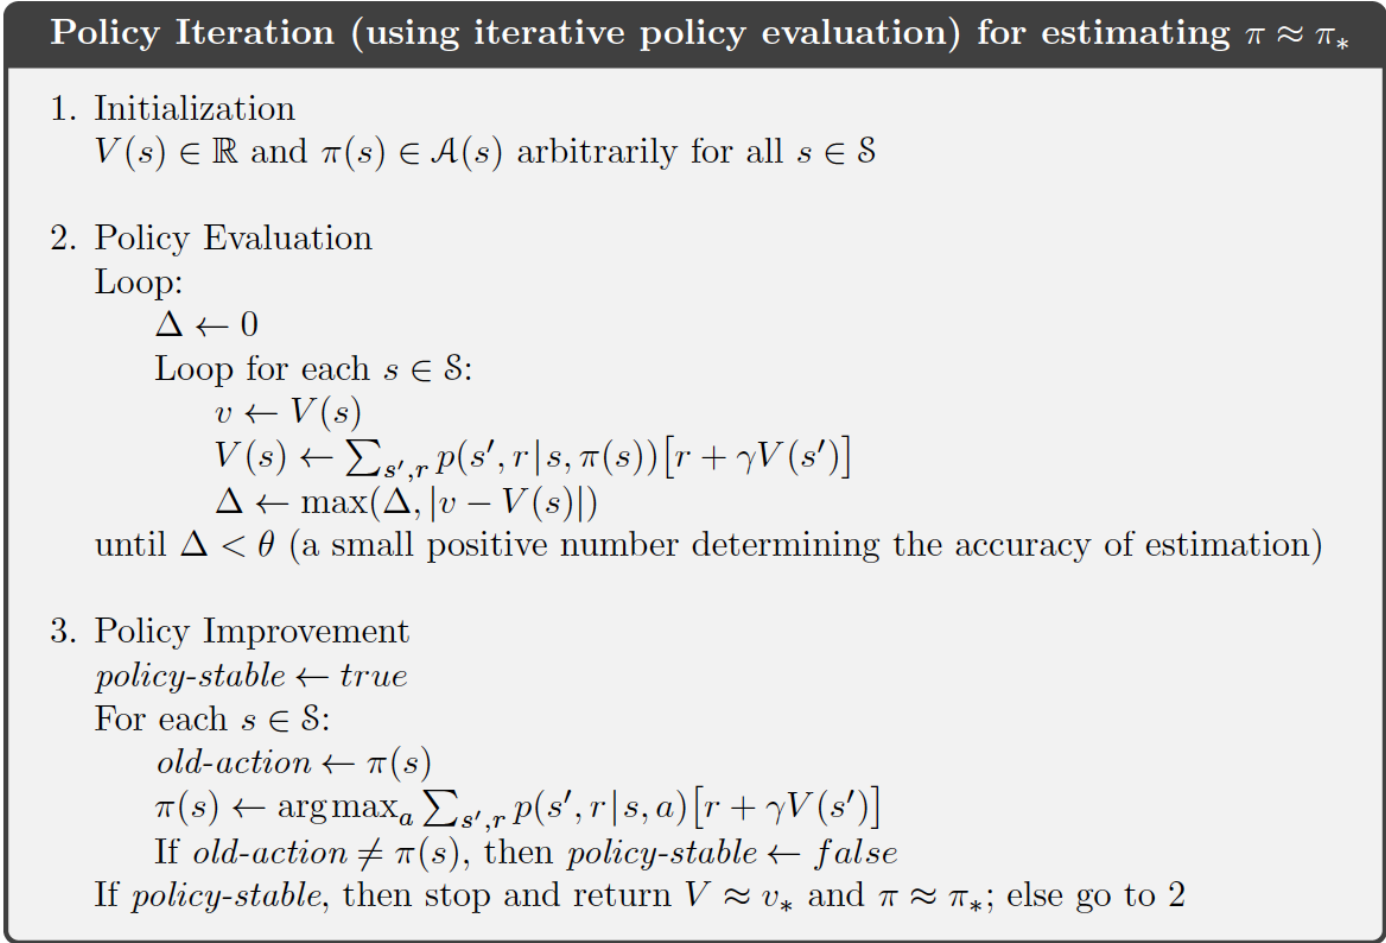
\includegraphics[width=0.55\textwidth]{./figure/policy_iteration_pseudocode}
    \vspace{-0.5cm}
\end{figure}

The results are shown as follows:
\begin{figure}[h]
    \centering
    \vspace{-0.2cm}
    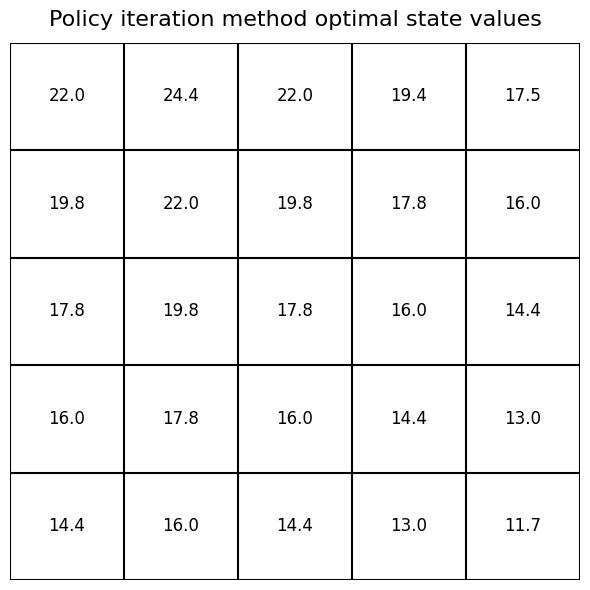
\includegraphics[width=0.45\textwidth]{./figure/p3_output/optimal/policy_iteration/V_value.png}
    \vspace{-0.5cm}
\end{figure}
\begin{figure}[h]
    \centering
    \vspace{-0.3cm}
    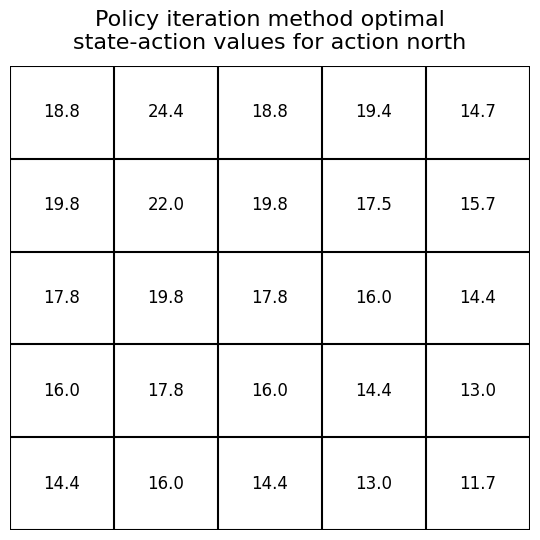
\includegraphics[width=0.45\textwidth]{./figure/p3_output/optimal/policy_iteration/Q_north.png}
    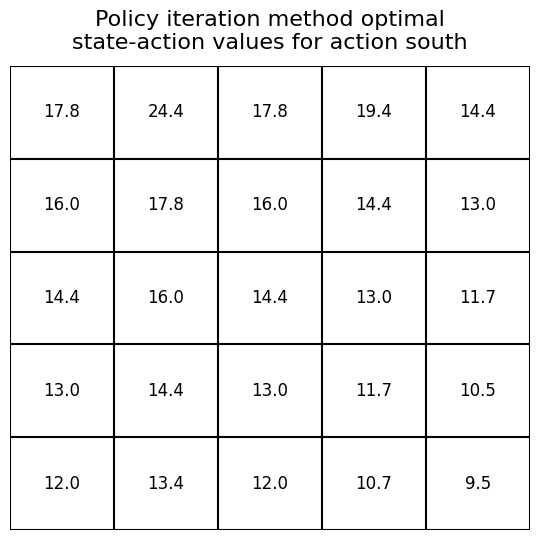
\includegraphics[width=0.45\textwidth]{./figure/p3_output/optimal/policy_iteration/Q_south.png}
    \vspace{-0.5cm}
\end{figure}
\begin{figure}[!htbp]
    \centering
    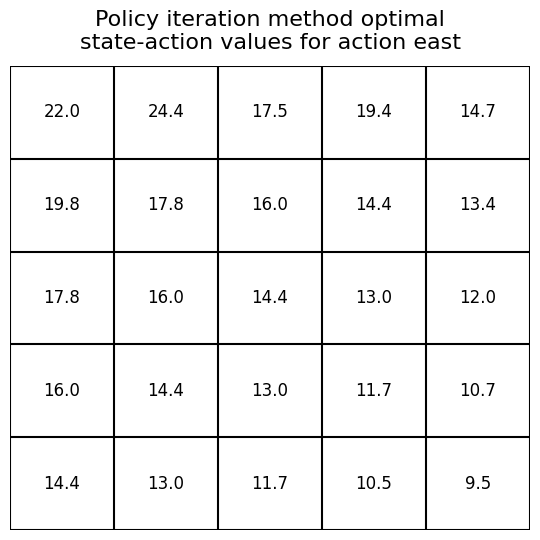
\includegraphics[width=0.45\textwidth]{./figure/p3_output/optimal/policy_iteration/Q_east.png}
    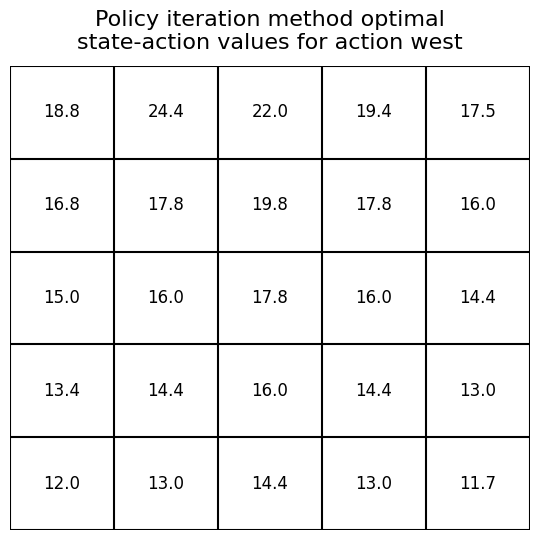
\includegraphics[width=0.45\textwidth]{./figure/p3_output/optimal/policy_iteration/Q_west.png}
    \vspace{-0.5cm}
\end{figure}
\begin{figure}[!htbp]
    \centering
    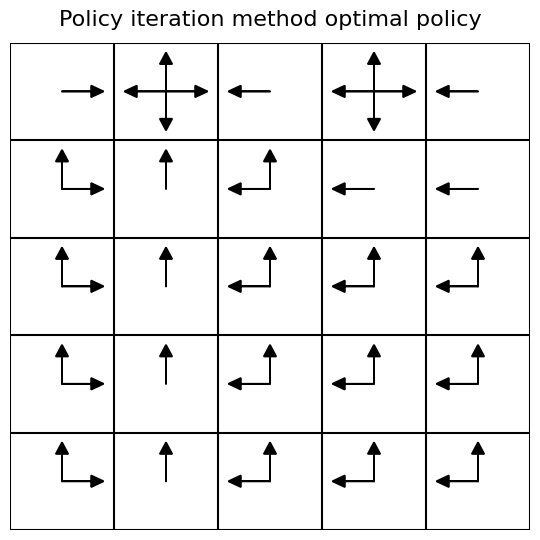
\includegraphics[width=0.4\textwidth]{./figure/p3_output/optimal/policy_iteration/policy.png}
\end{figure}

3. Value iteration method: \\
We can applying policy iteration method through the following pseudocode to get $v_*(s)$ and $q_*(s,a)$, then get $\pi_*(s)$ through $q_*(s,a)$:
\begin{figure}[!htbp]
    \centering
    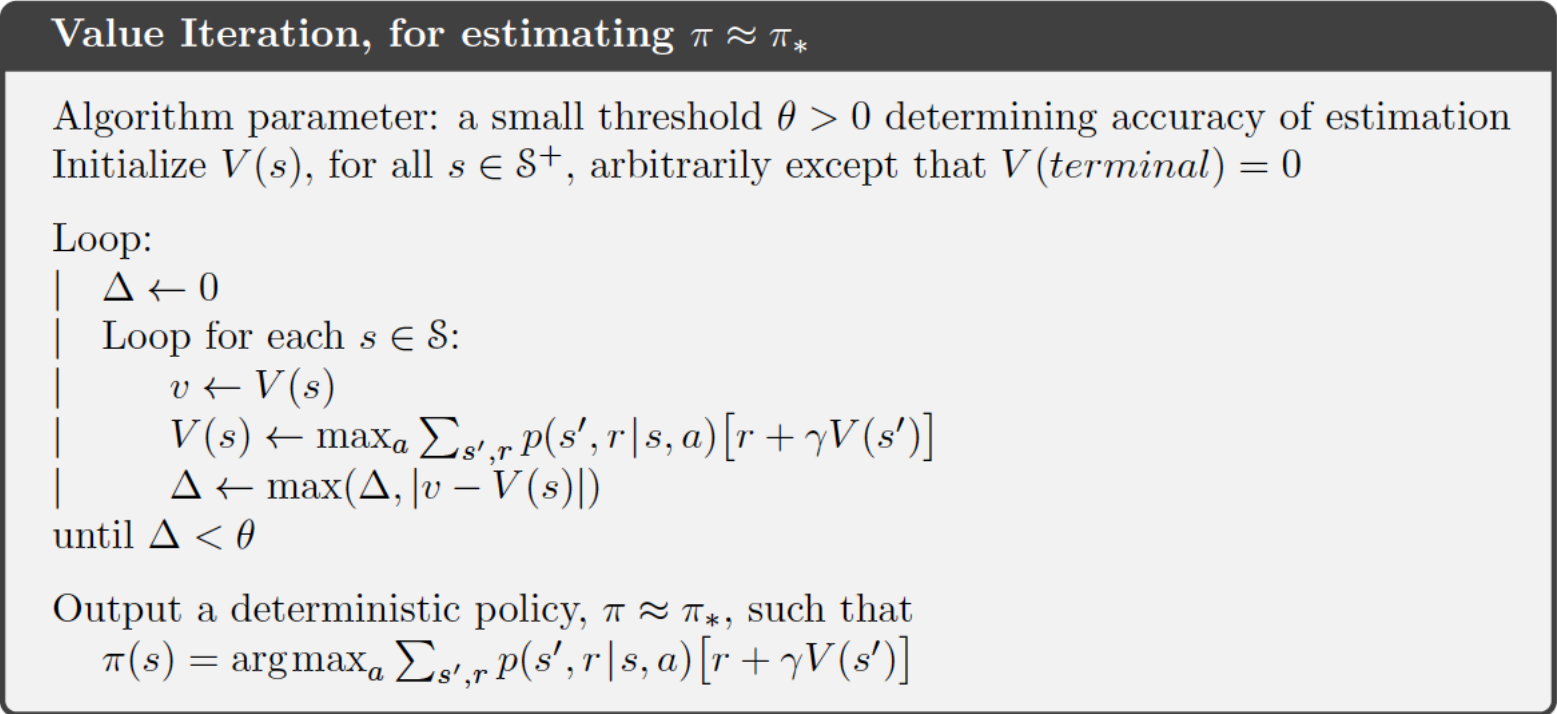
\includegraphics[width=0.7\textwidth]{./figure/value_iteration_pseudocode}
\end{figure}

The results are shown as follows:
\begin{figure}[!htbp]
    \centering
    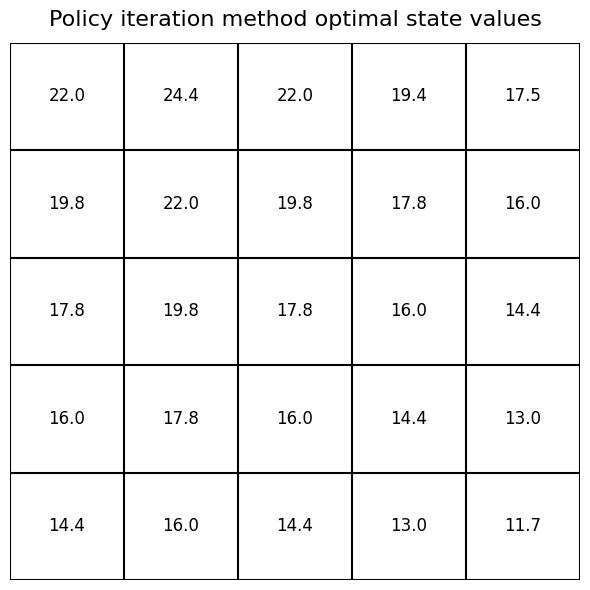
\includegraphics[width=0.45\textwidth]{./figure/p3_output/optimal/policy_iteration/V_value.png}
    \vspace{-0.5cm}
\end{figure}
\begin{figure}[h]
    \centering
    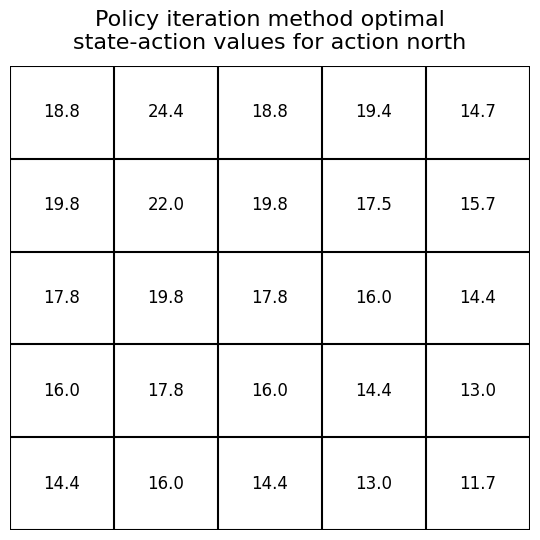
\includegraphics[width=0.45\textwidth]{./figure/p3_output/optimal/policy_iteration/Q_north.png}
    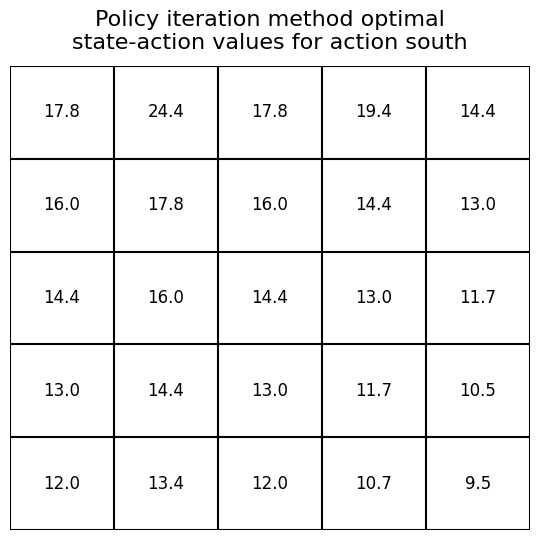
\includegraphics[width=0.45\textwidth]{./figure/p3_output/optimal/policy_iteration/Q_south.png}
\end{figure}
\begin{figure}[h]
    \centering
    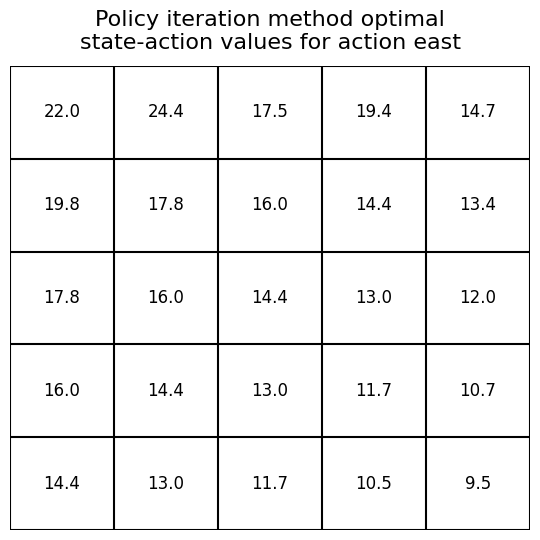
\includegraphics[width=0.45\textwidth]{./figure/p3_output/optimal/policy_iteration/Q_east.png}
    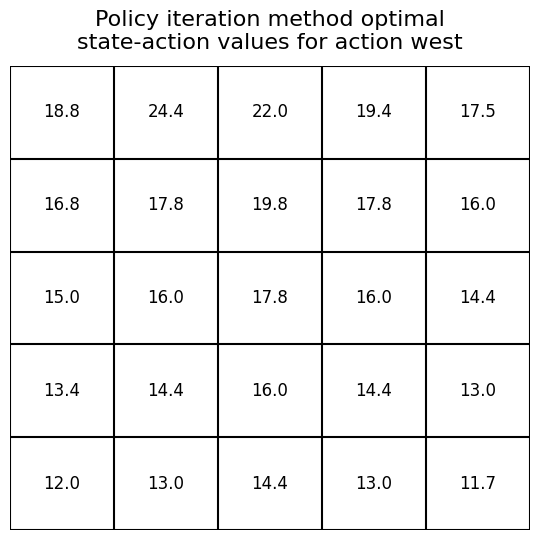
\includegraphics[width=0.45\textwidth]{./figure/p3_output/optimal/policy_iteration/Q_west.png}
    \vspace{-0.2cm}
\end{figure}
\begin{figure}[!htbp]
    \centering
    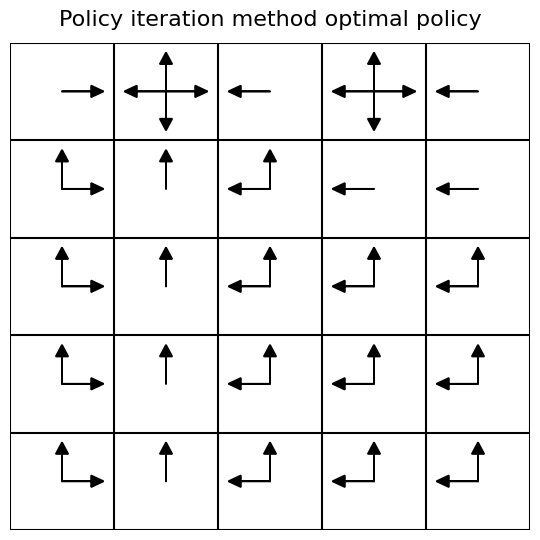
\includegraphics[width=0.4\textwidth]{./figure/p3_output/optimal/policy_iteration/policy.png}
\end{figure}

\end{homeworkProblem}

\newpage